
\section*{练习}
\label{sec:ch04-exercises}

\vkexsync{16}

\begin{exercise}\label{ex:ch04-16}
$S^2\times S^2$ 上是否存在一个\trMorseFunction，它有一个极小点、一个极大点与一个\trIndex{}为 2 的\trCriticalPoint，而其余诸\trCriticalPoint{}的\trIndex{}全都是 1 或 3？
\end{exercise}

\begin{exercise}\label{ex:ch04-17}
证明：复\trProjectiveSpace{} $\CP^n(\CC)$ 是\trSimplyConnected{}的。
\end{exercise}

\begin{exercise}\label{ex:ch04-18}
\cref{ex:ch01-08}的那个\trQuadric{} $Q$ 是否\trDiffeomorphic{}于 $\CP^2(\CC)$？我们把 $\CP^1(\CC)\times\CP^1(\CC)$ 用
\[
\bigl([a,b],[u,v]\bigr)\longmapsto[au,bu,av,bv]\text{。}
\]
送入 $\CP^3(\CC)$。证明：这是一个\trEmbedding，它的\trImage{}由方程
\[
z_0z_3-z_1z_2=0\text{。}
\]
所描述。再证明：$Q$ \trDiffeomorphic{}于 $S^2\times S^2$。
\end{exercise}

\begin{exercise}\label{ex:ch04-19}
\cref{fig:diffeomorphism-graph}画出了一个\trDiffeomorphism
\[
\varphi:\;]-1,1[\;\longrightarrow\;]-1,1[\text{。}
\]
的图像。我们令 $a=\varphi(0)$。证明：$\varphi$ 是 $]-1,1[$ 上某个\trVectorField{}在时刻 1 的\trFlow，并画出这个\trVectorField。设 $D$ 是 $\RR^N$ 中以 $0$ 为中心、半径为 1 的\trOpen{}\trDisk，并设 $a\in D$。构造 $D$ 上的一个\trVectorField，使其\trFlow{}满足 $\varphi^1(0)=a$。
\end{exercise}

\setcounter{figure}{11}%
\begin{figure}[htbp]
\centering
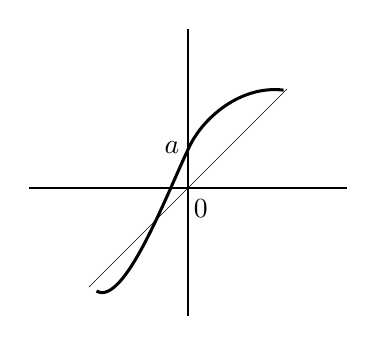
\begin{tikzpicture}[line width=0.6pt,scale=1.35]
  \draw (-1.50,0) -- (1.50,0);
  \draw (0,-1.20) -- (0,1.50);
  \draw[very thin] (-0.93,-0.93) -- (0.93,0.93);
  \draw[line width=1.1pt] (-0.86,-0.97)
        .. controls (-0.60,-1.12) and (-0.20,-0.06) .. (0,0.36)
        .. controls (0.13,0.66) and (0.50,0.97) .. (0.90,0.92);
  \node at (-0.15,0.38) {$a$};
  \node at (0.12,-0.19) {$0$};
\end{tikzpicture}
\caption{}
\label{fig:diffeomorphism-graph}
\end{figure}

\begin{figure}[htbp]
\centering
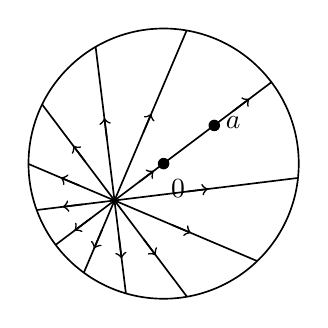
\begin{tikzpicture}[line width=0.6pt,scale=1.3]
  \begin{scope}
    \clip (0,0) circle (1.32);
    \foreach \a in {7,37,67,97,127,157,187,217,247,277,307,337}
      \draw (-0.48,-0.36) -- ++(\a:2.4);
  \end{scope}
  \draw (0,0) circle (1.32);
  \foreach \a/\s in {7/0.72, 67/0.72, 97/0.61, 127/0.47, 157/0.37, 187/0.31,
                     217/0.29, 247/0.31, 277/0.37, 307/0.47, 337/0.61}
    \draw[->] (-0.48,-0.36) ++(\a:\s) -- ++(\a:0.2);
  \draw[->] (-0.48,-0.36) ++(37:0.30) -- ++(37:0.18);
  \draw[->] (-0.48,-0.36) ++(37:1.45) -- ++(37:0.2);
  \fill (0,0) circle (1.6pt);
  \fill (0.495,0.373) circle (1.6pt);
  \node at (0.14,-0.24) {$0$};
  \node at (0.68,0.40) {$a$};
\end{tikzpicture}
\caption{}
\label{fig:disk-vector-field}
\end{figure}

\begin{exercise}\label{ex:ch04-20}
若 $u:V\to W$ 是一个 $\cC^\infty$ 映射，而 $V$ 与 $W$ 是\trCompact{}\trConnected\trManifold，则
\[
u_\star:HM_0(V;\ZZ/2)\longrightarrow HM_0(W;\ZZ/2)
\]
是一个\trIsomorphism（它是恒等映射，因为这两个空间都与 $\ZZ/2$ \trIsomorphic）。
\end{exercise}

\begin{exercise}\label{ex:ch04-21}
设 $V$ 是一个维数为 $n$ 的无边界\trCompact{}\trConnected\trManifold，并设 $D$ 是\trEmbedding{}于 $V$ 中的一个维数为 $n$ 的\trDisk。证明：
\[
HM_n\bigl(\overline{V-D};\ZZ/2\bigr)=0\text{。}
\]
由此推出：若 $u:V^n\to W^n$ 是一个 $\cC^\infty$ 映射，它诱导出一个\emph{非零}映射
\[
u_\star:HM_n(V;\ZZ/2)\longrightarrow HM_n(W;\ZZ/2)\text{，}
\]
则它是\trSurjective。
\end{exercise}

\begin{exercise}\label{ex:ch04-22}
设 $W$ 是一个维数为 $n+1$ 的\trCompact{}\trManifoldWithBoundary，并设 $V$ 为它的边界，即 $V=\partial W$。假定 $V$ 是\trConnected{}的：
\begin{enumerate}[label=(\arabic*)]
\item 证明：包含映射 $V\subset W$ 诱导出从 $HM_n(V;\ZZ/2)$ 到 $HM_n(W;\ZZ/2)$ 的零映射。
\item 由此推出：若 $u:V\to Z$ 是一个从 $V$ 到同维数的\trManifold{} $Z$ 的 $\cC^\infty$ 映射，而它在\trHomology{} $HM_n$ 上诱导的映射 $u_\star$ 非零，则 $u$ 不可能被延拓成一个映射 $\widetilde{u}:W\to Z$。
\item 特别地，不存在任何从 $W$ 到它的边界、且限制在边界上为恒等映射的映射（也就是说，一个收缩）。$W=D^{n+1}$ 的情形就是\trBrouwer{}定理的情形。
\end{enumerate}
\end{exercise}

\begin{exercise}\label{ex:ch04-23}
设 $V$ 是一个\trCompact\trManifold。证明：不存在从 $V$ 到它的任何真子集上的收缩（如有必要，参见\cref{subsec:brouwer-via-homology}）。\footnote{译注：本练习按字面为假：任取一点 $p\in V$，常映射 $r\colon V\to\{p\}$ 便是到真子集 $\{p\}$ 上的收缩（$r\circ j=\mathrm{Id}$）。疑原书本意是变形收缩（deformation retract），且还须补“无边界”等前提——例如 $D^n$ 变形收缩到它的中心点，仍是到真子集上的变形收缩；此处照原书排印，存疑备案。——译者注}
\end{exercise}

\begin{exercise}\label{ex:ch04-24}
对于\cref{ex:ch01-06}中所考虑的那个\trMorseFunction{} $f$ 以及 $\CP^2(\RR)$ 上的一个\trPseudogradient{}场 $X$，描述诸\trStableManifold{}与诸\trUnstableManifold，连同它们的\trOrientation{}与\trCoorientation。计算\trComplex{} $(C_\star(f;\ZZ),\partial_X)$ 的\trHomology。证明：\footnote{译注：原书此处左端印作 $HM_k\bigl(\CP_2(\RR);\ZZ\bigr)$（$\CP$ 带下标）；与同句正文 $\CP^2(\RR)$ 的上标写法相抵，系显见排印笔误；此处径改上标。——译者注}
\[
HM_k\bigl(\CP^2(\RR);\ZZ\bigr)=
\begin{cases}
\ZZ & \text{若 } k=0\text{，}\\
\ZZ/2 & \text{若 } k=1\text{，}\\
0 & \text{其余情形。}
\end{cases}
\]
\end{exercise}

\begin{exercise}\label{ex:ch04-25}
考虑 $S^n$ 的这样一个\trCellularDecomposition：它在每个维数上都恰有两个\trCellular，其中一个是另一个在\trAntipodal{}映射下的像。确定 $\CP^n(\RR)$ 上诱导的\trCellular\trComplex{}（如\cref{subsec:complexes-cellular-homology}中所定义）的\trDifferential{} $\partial$。计算 $HM_k(\CP^n(\RR);\ZZ/2)$。在 $\CP^n(\RR)$ 的每个\trCellular{}上取定一个\trOrientation，并用同样的方法计算 $HM_k(\CP^n(\RR);\ZZ)$。
\end{exercise}
